\PassOptionsToPackage{hyphens}{url}
\documentclass{article}
\makeatletter
\def\input@path{{../templates/iclr2027/source/iclr2027/}}
\makeatother
\usepackage{iclr2027_conference,times}
\usepackage[T1]{fontenc}
\usepackage{microtype,amsmath,amssymb,amsthm}
\usepackage{booktabs,tabularx,array,enumitem,flafter}
\usepackage{graphicx,etoolbox}
\usepackage[hidelinks]{hyperref}
\usepackage{url}
\urlstyle{same}
\setlength{\emergencystretch}{2em}
\newtheorem{proposition}{Proposition}
\newcommand{\oc}{OpenCorvus}
\newcommand{\code}[1]{\texttt{\nolinkurl{#1}}}
\newcommand{\yes}{\mathsf{S}}
\newcommand{\no}{\mathsf{R}}
\newcommand{\unk}{\mathsf{U}}
\newcolumntype{Y}{>{\raggedright\arraybackslash}X}
\title{\raggedright OpenCorvus: Evolving Expert Organizations for Professional Work}
\author{Author identities to be supplied before submission}
% Internal draft status only; official files, geometry and type sizes remain unchanged.
\makeatletter
\patchcmd{\@maketitle}{Anonymous authors}{Author identities pending}{}{\errmessage{Draft author status patch failed}}
\patchcmd{\@maketitle}{Paper under double-blind review}{Working manuscript with preliminary results}{}{\errmessage{Draft review status patch failed}}
\makeatother
\begin{document}
\maketitle
\lhead{Working manuscript, 11 September 2026; not submitted}
\begin{abstract}
Professional agent systems must carry specialized procedures across assignments and improve those procedures without losing the ability to identify what was executed and evaluated. We introduce Evolving Expert Organizations (EEOs), a framework that makes a reusable expert organization the unit of specialization and revision. Implemented in OpenCorvus, an organization packages role instructions, collaboration graphs, capability allocations, domain resources, and exact version identity. Domain specialization binds this structure to professional procedures and output contracts. An outer improvement process attributes failures from task evidence, constructs candidate revisions, and compares them with their parent under matched execution conditions. We define the admissible organizational update space and instantiate it with experience-driven procedural text revision while preserving executable resources and inherited capability references. Task-local execution remains bound to its original revision, and retained updates apply to subsequent work. Our analysis connects organizational improvement to search-cost amortization and independent evaluation after selection. A preliminary AutomationBench run of OpenCorvus Mission Base with GPT-5.6 Luna is recorded at 34\% strict pass over 100 workflows. This aggregate characterizes the execution harness; incomplete case-level provenance and the absence of matched ablations limit attribution to organizational mechanisms. The framework provides a concrete basis for investigating how professional agent organizations accumulate useful procedures across tasks.
\end{abstract}
\section{Introduction}
Professional work is organized around persistent responsibilities: a researcher collects evidence, an analyst transforms it, a reviewer checks the resulting claims, and a writer produces a deliverable. The organization carries procedures, tools, and handoff conventions from one assignment to the next. For a large language model (LLM) system, reproducing this arrangement requires more than assigning expert names. An analyst needs the correct computation tools and input resources; a reviewer needs the actual revision under review; and improvements discovered during one assignment must survive beyond its conversation.

We introduce \emph{Evolving Expert Organizations} (EEOs), a framework for representing, specializing, executing, and revising reusable agent organizations. Its implementation in \oc{} treats an expert organization as a versioned package containing role instructions, capability allocations, task-level collaboration graphs, and domain resources. A task binds to an exact package revision. An outer improvement process constructs a new revision from recorded experience and compares it with its parent on matched tasks. The resulting object of reuse is the organization, including its procedures and executable resource closure.

Consider a research report whose calculations are correct but whose prose uses an earlier result. Repairing that report addresses one assignment. Refining the writer's procedure so that each numerical claim is explicitly bound to its canonical result and revision-specific review targets a recurring organizational failure. The latter is an organizational update only when it is retained in a package and applied to subsequent tasks. Whether it improves those tasks is a separate, measurable question. This distinction connects the representation, update mechanism, and evaluation throughout the paper.

The paper makes three contributions. First, we define a portable organization representation that separates reusable expertise from task-local state and gives domain specialization an explicit resource and output contract. Second, we define a constrained revision protocol that connects the mutation surface, matched parent--candidate evaluation, and retained version-specific evidence. Third, we report a preliminary AutomationBench execution result and identify the evidence needed to attribute future changes to collaboration, specialization, or retained updating. Our technical analysis concerns the organizational mechanisms; the available experiment characterizes Mission Base and does not isolate those mechanisms.

\section{Related Work}\label{sec:related}
\paragraph{Expert collaboration.}
Role specialization and structured communication are established design choices. AutoGen supplies configurable conversational agents, and MetaGPT uses professional roles and operating procedures to coordinate software work \citep{autogen,metagpt}. EEO makes the portable package the unit of specialization and revision: roles are coupled to their capability references, supporting resources, and handoff declarations. Neither the use of expert roles nor a dependency graph alone constitutes the contribution.

\paragraph{Automatic agent and workflow design.}
EvoAgent mutates agent settings, selects diverse offspring with an LLM quality check, and integrates their task outputs \citep{evoagent}. AFlow represents workflows in code and uses execution feedback in a variant of Monte Carlo tree search \citep{aflow}. ADAS uses a meta agent to program new agents from an archive of prior designs and evaluations, including transfer across tasks, domains, and models \citep{adas}. These results motivate treating organizational revision as search, but they preclude claiming that automatic design or cross-task reuse originates here. EEO studies a constrained package search space that carries domain resources and capability allocations together with instructions. Its current generator edits the procedural layer; broader structural edits are represented and checked by the package integrity interface.

\paragraph{Reflective prompt optimization.}
GEPA (Genetic-Pareto) already uses execution feedback to revise module prompts, retain candidates, and optimize held-out performance with fixed model weights \citep{gepa}. EEO's text configuration therefore does not introduce reflection-based optimization. Its contribution concerns professional organization packaging, explicit resource boundaries, and attributable revision retention. A matched optimizer comparison on this substrate is needed to attribute benefits to the particular revision policy.

\paragraph{Learning from experience.}
SiriuS retains successful reasoning trajectories, augments unsuccessful ones, and performs supervised fine-tuning of individual agent models \citep{sirius}. EEO holds the foundation model fixed and retains improvements in organization packages. The two update different objects and can be combined, but an experience archive by itself does not establish learning: a retained package change and its measured transfer are the relevant evidence here.

\paragraph{Procedural memory and versioned improvement.}
LEGOMem distills successful trajectories into full-task and agent-specific memories and retrieves them for the orchestrator and task agents \citep{legomem}. It directly addresses reusable procedural knowledge in multi-agent workflows. EEO instead revises a package's standing instructions and resources; cross-task procedural reuse is common to both. AgentDevel externalizes agent revision into a versioned development process with executable diagnosis, candidate evaluation, and regression-aware selection \citep{agentdevel}. Thus, external improvement and traceable version retention are also established ideas. EEO's specific design couples the professional organization to an explicit text mutation surface and inherited resource declarations. This combination motivates comparative study; it does not establish superiority over memory retrieval or other revision policies.

\paragraph{Enterprise harness evolution.}
StarHarness revises environment-specific harnesses with fixed model weights, a candidate ledger, development traces, and separate selection and holdout roles; its experiments include AutomationBench Finance \citep{starharness}. Its editable space includes executable interfaces and agent-loop configuration. EEO's present text study holds those resources fixed. A fair comparison must disclose this difference in editable space. Enterprise harness evolution and its evaluation on AutomationBench are prior contributions; the preliminary Mission Base result does not supply such a head-to-head comparison.

\paragraph{Execution substrate.}
Agent environments and interfaces, exemplified by SWE-agent and OpenHands, determine how agents interact with tools and artifacts \citep{sweagent,openhands}. The OpenHands Software Agent SDK also provides persistent event-oriented execution \citep{ohsdk}. EEO uses exact package binding and revision-specific artifacts to keep organizational comparisons attributable. These supporting mechanisms do not by themselves imply better reasoning or semantic correctness.

\section{Executable Expert Organizations}\label{sec:organization}
\subsection{Representation and execution}
An organization revision is
\begin{equation}
\mathcal O_v=(R_v,G_v,P_v,K_v,A_v,F_v;\,h_v).
\label{eq:organization}
\end{equation}
$R_v$ is the set of expert roles. $G_v$ is a collection of directed acyclic graphs whose nodes name roles and whose edges declare task-level dependencies. $P_v$ contains the orchestrator and expert instructions. $K_v$ contains model-readable skills, procedures, references, and examples. $A_v$ maps the orchestrator and roles to declared capability references, including tools and skills. $F_v$ is the complete package file set, containing these resources and any executable or opaque assets. The content digest $h_v$ identifies the exact revision; a human-readable version label is additional metadata.

A role may occur in different workflow declarations, so roles and workflow nodes are distinct objects. The graphs expose intended dependencies to the orchestrator. Dispatch remains an LLM decision using predecessor evidence, active workers, and execution capacity; graph validity is not a proof that every dependency is semantically satisfied at runtime.

For task $x$, execution produces a trajectory $\tau$ and deliverable $y$:
\begin{equation}
(\tau,y)\sim \operatorname{Run}_{\phi}
   (\mathcal O_v,x,\eta,b).
\label{eq:run}
\end{equation}
Here $\phi$ fixes the foundation model and inference configuration, $\eta$ specifies the workspace, tools, permissions, and external environment, and $b$ is the task budget. The task stores an immutable package binding. Worker descriptors carry the corresponding projected capabilities and revision identity. Conversation state, intermediate artifacts, and scheduler ownership belong to the execution, rather than to the reusable organization.

Figure~\ref{fig:organization} shows the representation through the Research Studio package. Its five expert roles cover planning, research, analysis, fact checking, and writing. The analyst produces canonical computation evidence before fact checking; the writer renders the accepted evidence rather than recomputing numerical claims. These are declared responsibilities and workflow relationships in the inspected package \citep{ocsource}.

The same package declares three workflows with different entry conditions. Full research uses all five roles when the assignment requires new source collection. Evidence synthesis starts with the analyst when a sufficient source bundle is already supplied. Direct writing uses the writer alone for bounded material that requires faithful presentation without new research claims. These alternatives reuse the same role definitions and resources; they do not require a separately maintained organization for each task shape. Choosing among them remains part of the orchestrator's task interpretation. A task with missing computational evidence cannot become a direct-writing task merely by asking the writer to supply the missing calculations.

\begin{figure}[!t]
\centering
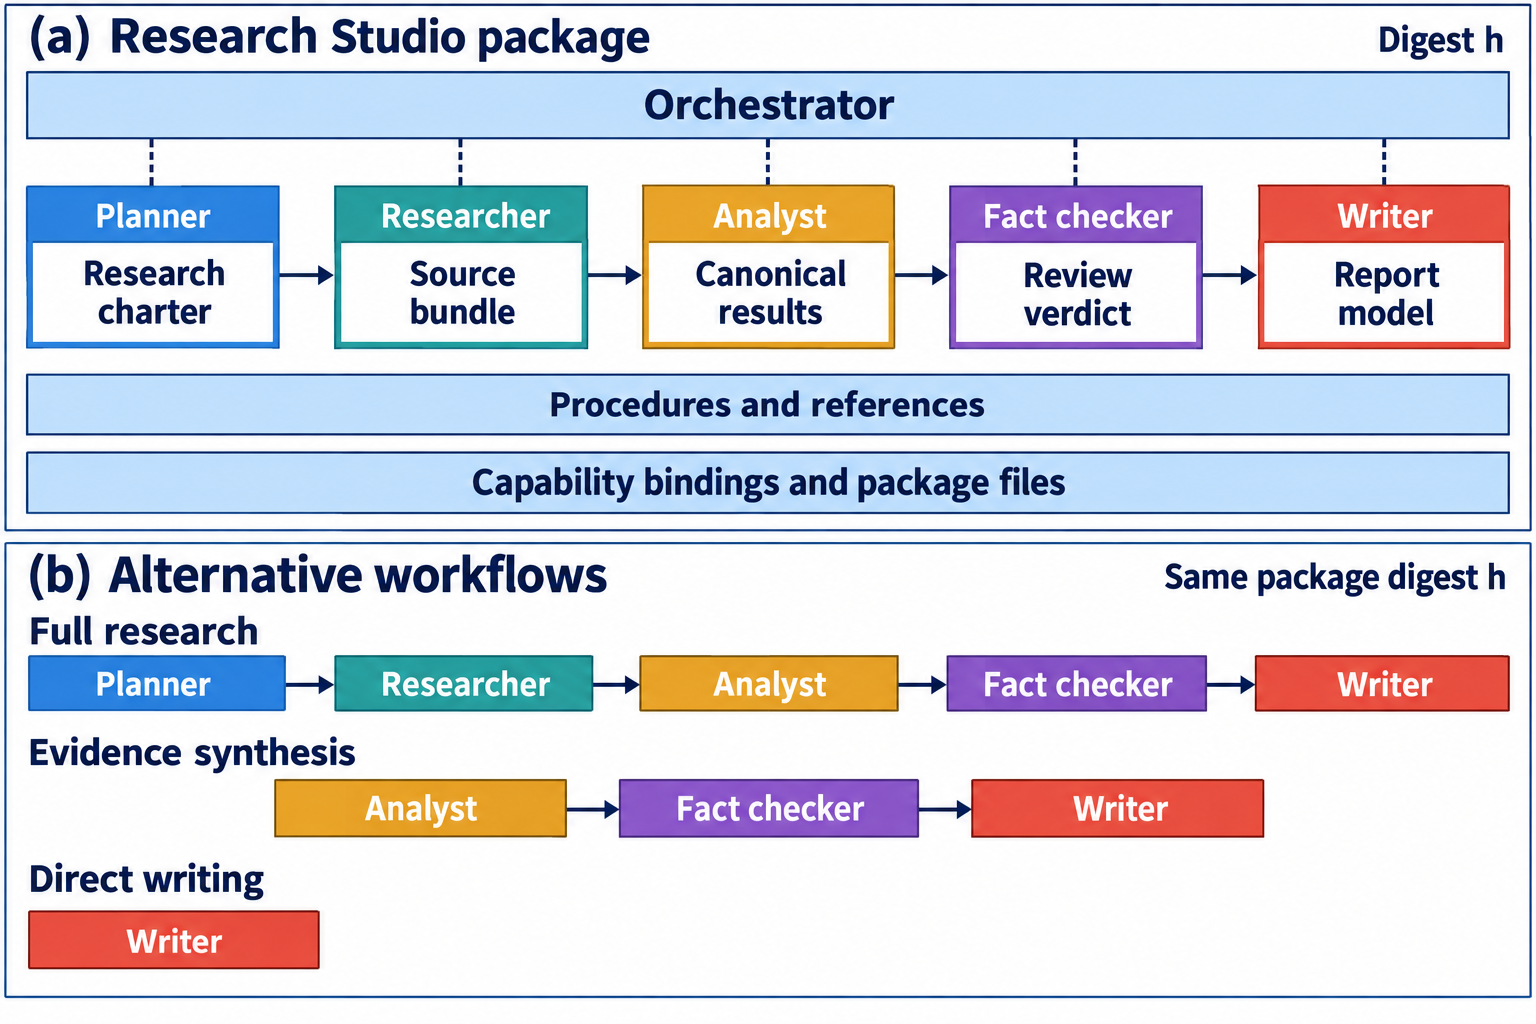
\includegraphics[width=\linewidth]{figures/architecture.png}
\caption{A reusable organization and its task-specific workflow choices. The five expert roles, their output types, and the three alternative workflow declarations follow Research Studio. The image abbreviates the package digest $h_v$ as $h$. Solid role-to-role arrows are declared dependencies; dashed orchestrator links indicate LLM dispatch. The resource bands belong to the package, while outputs and execution state belong to individual tasks.}
\label{fig:organization}
\end{figure}


\subsection{Domain specialization}
We express a domain specification as $\mathcal D=(\mathcal X,K^{\mathcal D},A^{\mathcal D},C^{\mathcal D},q^{\mathcal D})$: a task family, domain procedures, required capabilities, output contracts, and an evaluation rubric. A specialization operation
\begin{equation}
\mathcal O^{\mathcal D}_0
  =\operatorname{Specialize}(\mathcal O_{\mathrm{base}},\mathcal D)
\label{eq:specialization}
\end{equation}
constructs a package with explicit role responsibilities and resource bindings. $C^{\mathcal D}$ and $q^{\mathcal D}$ are analytical names for the domain's artifact schemas, checking procedures, and scorers; they are not additional mandatory manifest fields.

For evidence-based analysis, specialization assigns collection and citation procedures to the researcher, executable calculations and canonical result schemas to the analyst, verification criteria to the fact checker, and a report template to the writer. The evaluation checks numerical agreement with the canonical results, claim support, and delivery requirements. Replacing the names with professional titles while keeping tools, procedures, and acceptance criteria unchanged is an insufficient specialization.

Initial specialization can introduce domain resources and authorized tools. Subsequent evolution operates within the parent package's inherited capability envelope and frozen executable resources. This separates establishing what an organization can access from learning how it uses those resources. It also makes the comparison with a fixed specialized organization meaningful: both start with the same professional substrate.


\subsection{A concrete professional contract}\label{sec:contract}
The analytical-report specialization gives organizational knowledge three connected forms. A \emph{procedure} explains how to perform a recurring operation, such as reconciling a source population before aggregating it. A \emph{resource binding} makes the corresponding input, tool, schema, or reference available to the responsible role. An \emph{artifact contract} describes the evidence a downstream role needs before using the output. These forms have different failure modes: good instructions cannot compensate for an unavailable source, and an available calculation tool does not specify which population or units are appropriate.

For a report task, the planner fixes the question, source hierarchy, comparison dimensions, and stopping conditions. The researcher assembles durable sources and identifies disagreement. The analyst records the calculation method, source identities, canonical tables, and claim-to-result correspondence. The fact checker examines those post-computation claims and records corrections and unresolved limits. The writer constructs a structured report model from the accepted material and derives its presentation from that model. This allocation follows the Research Studio instructions \citep{ocsource}. It places the numerical method upstream of verification and presentation, so a persuasive final report is not the only object available for inspection.

To make the handoff precise, consider a quantitative claim $\kappa$. Its analytical support record can be written as $(\kappa,r,a,\ell_{\mathrm{rev}})$, where $r$ identifies a canonical result revision, $a$ locates the relevant table cell or range, and $\ell_{\mathrm{rev}}$ identifies the review addressing that claim and result. This notation describes the information relationship, not a new mandatory runtime schema. A complete record still needs semantic checking: the table may use the wrong population, the cited range may not entail the prose, or the review may leave the claim unresolved. The writer's contract therefore concerns both locating the resources and preserving the accepted meaning, units, qualifications, and uncertainty.

The reusable package contains the rules for constructing and checking such relationships. Task-specific sources, computed values, and accepted conclusions remain in the task's evidence. Thus, specializing an organization for analytical reporting does not require installing the answer to each report in its prompts. It establishes a procedure that can be applied to different questions, source bundles, and result tables. Whether this procedure transfers well is measured on new tasks with separately constructed evidence.

\section{Experience-Driven Organizational Evolution}\label{sec:evolution}
The outer improvement process takes evaluated task evidence and a parent package as input, constructs candidate revisions, and retains the selected organization for subsequent tasks.

\subsection{Experience and attribution}
We represent the evidence associated with an evaluated execution as
\begin{equation}
e=(x_{\mathrm{id}},h_v,\gamma,\ell_{\tau},\ell_y,s,c,u,\iota),
\label{eq:experience}
\end{equation}
where $\gamma$ identifies the frozen evaluation context; $\ell_{\tau}$ and $\ell_y$ locate run evidence and deliverable resources; $s$ is a scorer vector; $c$ records resource consumption; $u$ records human intervention; and $\iota$ locates independent integrity review. This tuple joins the implementation's separate run, evaluation, resource, and review records; intervention time is an additional study measurement. Task and package identities make the evidence attributable to a particular revision.

The Evolution Lab divides improvement work among observation, failure analysis, experiment planning, candidate authoring, evaluation, integrity review, and recommendation roles. The failure analyst identifies a recurring procedural mismatch and links it to concrete runs. For the running example, the hypothesis is that obligations distributed across the writer instructions and quality skill need a more explicit local sequence where individual claims enter the report. A candidate elaborates the claim-to-result handoff procedure and its reference example. This attribution is a testable hypothesis, not a causal conclusion inferred solely from an LLM explanation.

\subsection{Candidate space and update policy}
A candidate $\mathcal O'$ must preserve the package's logical identity, declare a new version, and contain a substantive change. Let $\operatorname{Cap}(\mathcal O)$ denote the union of locally expanded capability references declared by its orchestrator and agents; let $\operatorname{Base}(\mathcal O)$ denote their base-role set. Same-package capability sets are expanded to member references; external references retain their encoded identity. The integrity relation requires
\begin{align}
\operatorname{Cap}(\mathcal O')&\subseteq\operatorname{Cap}(\mathcal O_v),
&
\operatorname{Base}(\mathcal O')&\subseteq\operatorname{Base}(\mathcal O_v),
\label{eq:capability}\\
F'|_{\overline{M}}&=F_v|_{\overline{M}},
&
M&=M(\mathcal O_v)\cup M(\mathcal O')\cup\{m\}.
\label{eq:frozen}
\end{align}
$M(\mathcal O)$ contains declared prompts, the package README and selector instructions, and eligible UTF-8 skill instructions, references, and examples. Here $m$ denotes the manifest path, handled as a mutable declaration. Equation~\ref{eq:frozen} requires both file-set equality and byte equality outside the two text closures and the manifest. Candidate validation additionally resolves declared prompt paths, workflow agents, and dependencies, and rejects cycles.

The representation admits four kinds of change: procedural text; redistribution of inherited capabilities; workflow dependencies; and the role roster. Figure~\ref{fig:specialization} develops a procedural candidate within a concrete professional specialization. The union constraint in Equation~\ref{eq:capability} is package-wide. A newly introduced role can receive a capability previously held elsewhere in the parent, so it is not a per-role non-escalation guarantee.

The released candidate author is instructed to edit procedural text:
\begin{equation}
\mathcal O'\sim
  \mu_{\phi}(\,\cdot\mid\mathcal O_v,\mathcal E_{\mathrm{dev}},H\,),
\label{eq:mutation}
\end{equation}
where $H$ is the attributed failure hypothesis. The intended text space $\mathcal S_{\mathrm{text}}(\mathcal O_v)$ fixes the role roster, topology, capability allocations, and declared resource paths. It permits eligible instructions and references and the descriptive manifest fields named by the released authoring policy: top-level name, label, and description; selector summary and selection guidance; and agent, workflow, and workflow-node labels and descriptions. These descriptions can affect selection and dispatch without changing the declared roles or edges. All other manifest fields are fixed except the version label. A prompt does not guarantee that every sampled proposal belongs to this space. The research arm therefore checks the realized diff against $\mathcal S_{\mathrm{text}}$ before admitting a candidate to its trials; rejected attempts still consume its budget. This arm-eligibility check is part of the experimental protocol, distinct from the broader production validator. Structural mutation is an extension supported by the representation and integrity interface, rather than an automatically explored operator in this configuration.

\subsection{Worked example: refining a claim handoff}\label{sec:worked}
Consider a development case in which an analyst publishes a corrected result after an earlier calculation, and a report incorporates a value from the earlier revision. The arithmetic in the corrected resource is sound, but the final numerical claim has the wrong evidential basis. This is an illustrative execution pattern for explaining candidate construction, not a reported experimental case. The current writer instructions already require exact analysis and review resources. The shared quality skill additionally requires claim identifiers, result-table coordinates, verification evidence, and a report model populated from accepted claims. The candidate therefore changes where and in what order these existing obligations are presented to the writer; it does not introduce the evidence contract itself.

The failure analyst first distinguishes competing explanations. The writer may have read an old resource; it may have read the correct resource but transcribed the wrong cell; or the report renderer may have consumed a stale report model. These explanations require different revisions. A run whose locators identify the accepted analysis but whose report-model claim points to a superseded table supports investigating the handoff procedure. A run whose model is correct but whose rendered document differs instead directs attention to the rendering path. The evidence narrows the candidate hypothesis; a fluent retrospective explanation alone does not identify the cause.

For the handoff hypothesis, the text candidate reorganizes those distributed obligations into a checklist placed at the writer's claim-construction step: open the accepted result; resolve the associated review; bind the claim to its table coordinate; and write the value together with its qualifications and unresolved limits. A companion example contrasts a corrected result with a superseded one using generic placeholders. This changes the presentation and point of use of the existing requirements, while preserving their underlying acceptance contract. The update retains the role roster, collaboration declarations, capabilities, and executable files. Its reusable content is the sequence of checks and the reference pattern, rather than a copied task answer or a task-specific source locator. Figure~\ref{fig:specialization} shows this relationship between specialization, evidence, and procedural revision.

The transfer hypothesis concerns the effect of that reorganization: tasks that require carrying revised quantitative evidence into a report should exhibit fewer result--report mismatches. The same procedure can also add retrieval and checking cost, cause excessive abstention when review evidence is partial, or distract from qualitative synthesis. Matched trials therefore examine contract satisfaction and resource use, and retention tasks include assignments for which the extra numerical procedure is irrelevant. If improvement occurs only on the development example, the evidence supports fitting that example rather than transferable organizational learning. If output correctness remains unchanged while checking cost rises, the revision can be valid and precisely attributable without being useful.

\begin{figure}[!t]
\centering
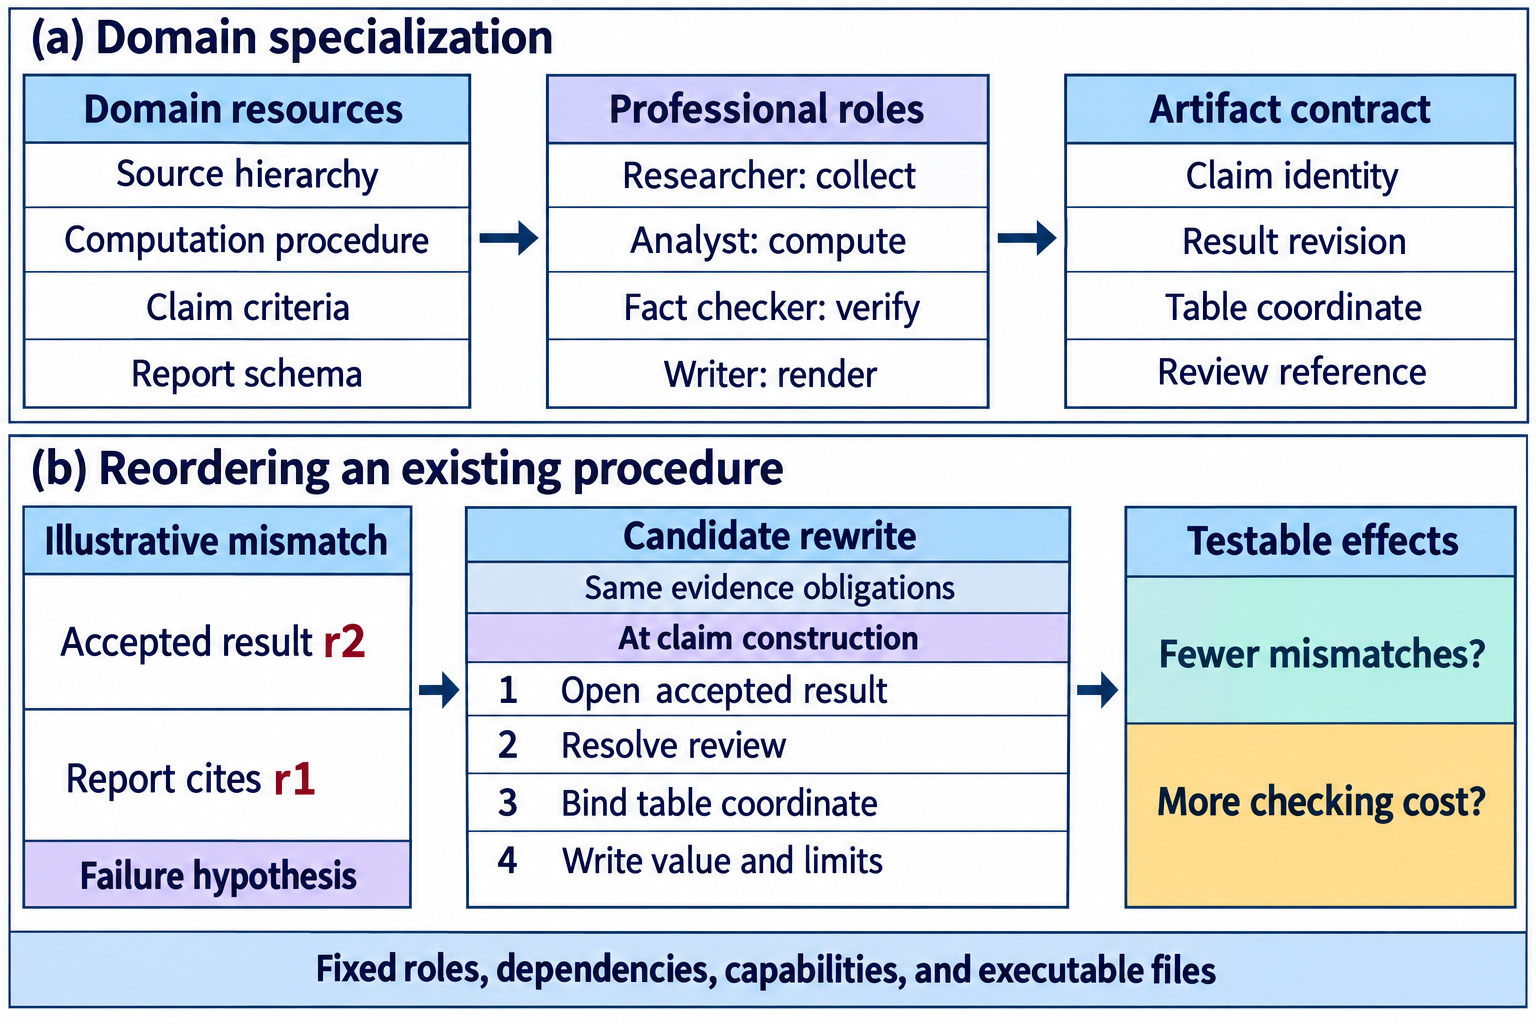
\includegraphics[width=\linewidth]{figures/specialization.png}
\caption{Domain resources and professional responsibilities support a shared analytical contract. The worked candidate reorganizes obligations already distributed across the writer prompt and shared quality skill into an explicit sequence at claim construction (Section~\ref{sec:worked}). The transfer hypothesis concerns this procedural reorganization; it does not establish a new evidence contract. The labels r1 and r2 denote illustrative superseded and accepted result revisions. The fixed-update footer describes the EEO--text research arm.}
\label{fig:specialization}
\end{figure}


\subsection{Matched comparison and retention}
A campaign fixes task cases, repetitions, scorer digests, model configuration, environment, permissions, arm order, and resource ceilings. Baseline and candidate executions occupy matched case--repetition slots and use their exact package revisions. The publisher derives candidate identities and file differences from validated resources. Evaluation results are projected from metric execution receipts, and independent integrity review binds to the exact evaluated revision.

For scorer $j$, let $s_{ij}^{a}$ be the value for slot $i$ and arm $a\in\{0,1\}$, with 0 denoting the parent. The comparison computes
\begin{equation}
d_{ij}=s_{ij}^{1}-s_{ij}^{0},\qquad
\bar d_j=\frac{1}{n}\sum_{i=1}^{n}d_{ij},\qquad
\widehat\Delta=\sum_j w_j\frac{\sigma_j\bar d_j}{|t_j-f_j|}.
\label{eq:comparison}
\end{equation}
Weights $w_j$ are the campaign's nonnegative weights normalized to sum to one, $\sigma_j\in\{-1,1\}$ sets the preferred direction, and distinct target and floor values $t_j,f_j$ define the scale. Missing required runs, scorers, or reviews make a comparison unavailable rather than contributing a zero score. The implementation reports paired summaries and an operational retain/select/inconclusive recommendation. Its multi-scorer interval approximation is discussed in Appendix~\ref{sec:implementation}; confirmatory inference uses the separate task-level analysis in Section~\ref{sec:analysis}.

Retention creates a traceable successor relation $\mathcal O_v\rightarrow\mathcal O_{v+1}$ and records the comparison context. Activation applies the selected revision to new tasks, preserving existing task bindings. A user-requested revision can also be retained through explicit feedback, but that path carries no claim of measured improvement. Selection, installation, and demonstrated learning therefore have distinct evidence.

Table~\ref{tab:algorithm} summarizes one complete improvement cycle. Candidate generation and matched comparison can repeat within the frozen development budget; the independent test partition is opened only after the final selection.


\begin{table}[htbp]
\centering\small
\begin{tabularx}{\linewidth}{@{}rY@{}}
\toprule
Step & One organizational improvement cycle \\
\midrule
1 & Freeze the parent package, development inputs, scorer versions, and total search budget. \\
2 & Inspect development run evidence; attribute a recurring failure and state a candidate hypothesis. \\
3 & Generate a text-policy candidate; check the realized diff for text-arm eligibility, then validate the package, inherited capabilities, and frozen files. Charge rejected attempts to search. \\
4 & Execute matched parent and candidate trials; collect metrics, failures, resource use, and independent integrity review. \\
5 & Record the comparison. Retain the parent or select an eligible candidate; keep each evaluated revision and its evidence addressable. \\
6 & Freeze the final selected revision before evaluation on unseen tasks and capability-retention tasks. Start later development with a fresh evaluation partition. \\
\bottomrule
\end{tabularx}
\caption{EEO improvement procedure. Steps 1--5 use Evolution Lab's package and evaluation interfaces. Step 6 specifies the research evaluation boundary; reuse of a test partition for subsequent candidate selection invalidates that boundary.}
\label{tab:algorithm}
\end{table}

\section{Analysis: What Constitutes Improvement?}\label{sec:analysis}
\begin{figure}[!t]
\centering
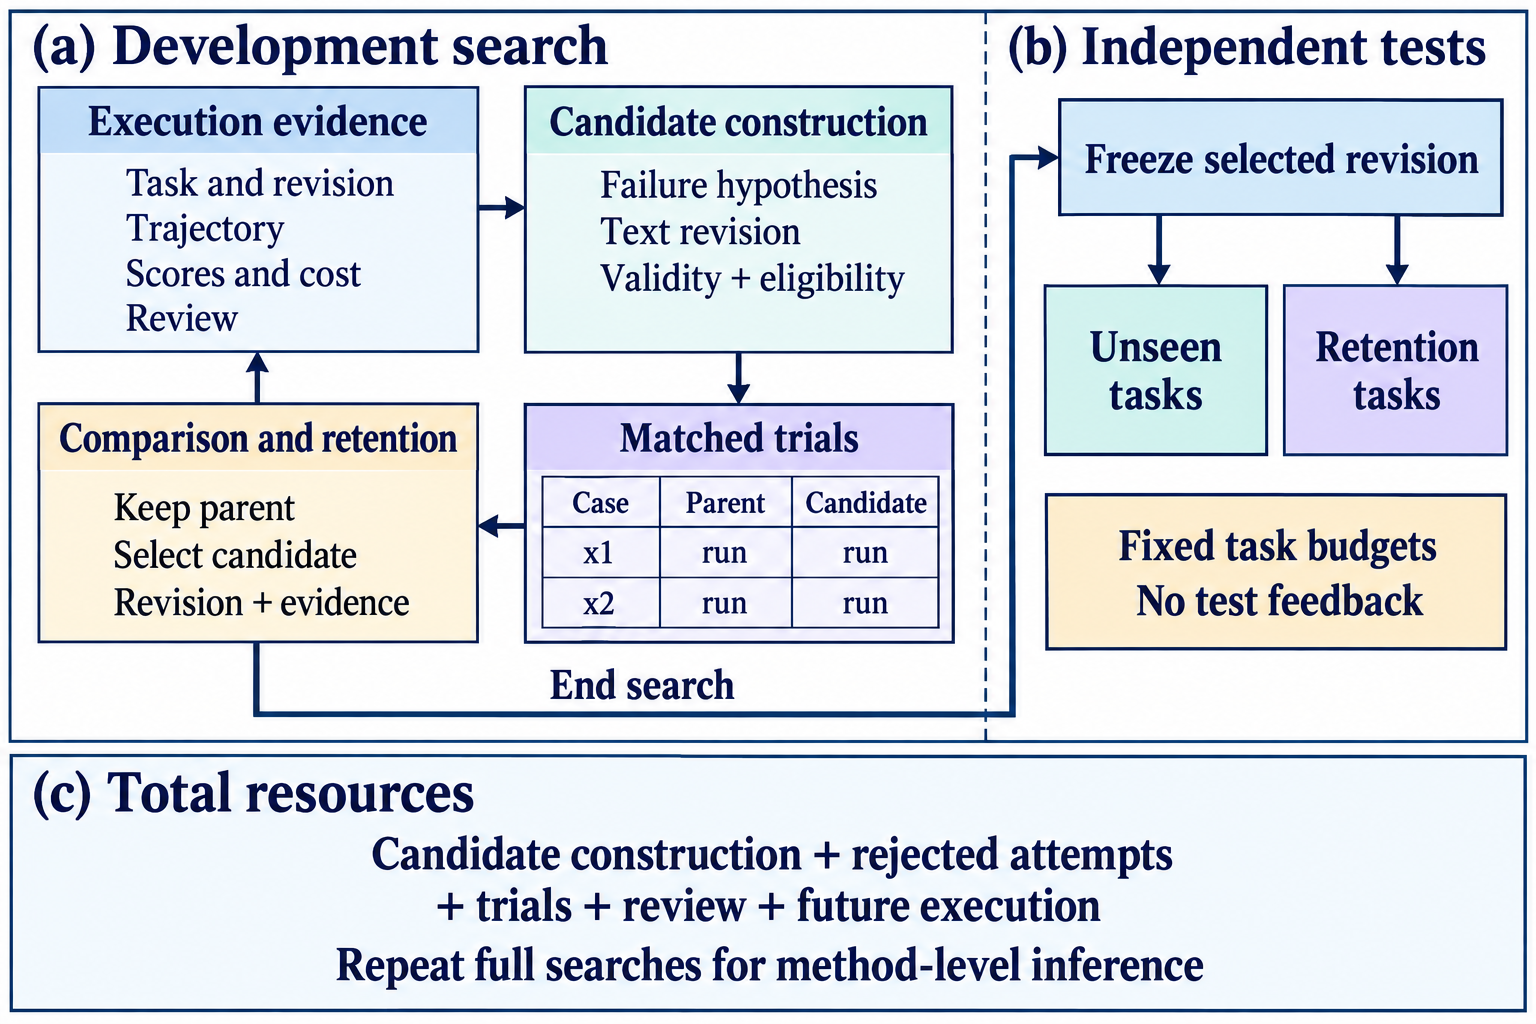
\includegraphics[width=\linewidth]{figures/evolution.png}
\caption{Evaluation design for retained organization revisions. Development trials support candidate construction and selection; frozen revisions are subsequently evaluated on separate future-task and retention sets. Trial cells depict comparisons, not measured results. All search and execution costs enter the accounting. Generalization over a search method requires independent search episodes and appropriate fresh partitions. This method diagram does not represent the protocol or outcomes of the preliminary Mission Base run in Section~\ref{sec:evaluation}.}
\label{fig:evolution}
\end{figure}

\subsection{Resource closure and revision isolation}
The inherited-reference constraint composes across retained revisions. If every transition satisfies Equation~\ref{eq:capability}, then, by transitivity of set inclusion, $\operatorname{Cap}(\mathcal O_v)\subseteq\operatorname{Cap}(\mathcal O_0)$ and likewise for base roles. Together with the frozen-file comparison, this bounds the resources an accepted candidate can introduce through this update path. It does not imply semantic safety: a changed instruction can misuse an existing tool, and a remote tool or externally resolved capability set can change without changing its reference.

Exact task binding also separates an update's intended unit of effect. Executions already bound to $h_v$ continue to identify $\mathcal O_v$; future tasks bound to $h_{v+1}$ identify the successor. This removes one source of attribution ambiguity, but it does not make the external environment stationary. Comparison contexts must still account for tool versions, model configuration, workspace state, and nondeterminism.

\subsection{Total value and amortization}
Let $q(\mathcal O,x)\in[0,1]$ measure task quality and let $c(\mathcal O,x)$ and $u(\mathcal O,x)$ measure execution cost and intervention time. For fixed nonnegative conversion weights $\lambda,\rho$, define per-task utility
\begin{equation}
U(\mathcal O,x)=q(\mathcal O,x)-\lambda c(\mathcal O,x)-\rho u(\mathcal O,x).
\label{eq:utility}
\end{equation}
Quality, cost, and time are also reported separately; the weights express an application-specific tradeoff rather than an intrinsic quality measure.

Suppose a revision has expected utility gain $g$ over its parent on the future task distribution, and the entire search and validation process costs $C_{\mathrm{search}}$ in the same utility units. Over $T$ tasks, its expected net advantage is
\begin{equation}
V_T=Tg-C_{\mathrm{search}},\qquad
V_T>0\ \Longleftrightarrow\ T>C_{\mathrm{search}}/g\quad(g>0).
\label{eq:amortization}
\end{equation}
This accounting identity explains why an improved task score is insufficient evidence of useful evolution. Search includes unsuccessful candidates, experiment planning, both trial arms, evaluator calls, and integrity review. When $g\leq0$, additional reuse cannot repay a nonnegative search cost under this stationary model. When tasks change over time, the relevant expression is $\sum_{t=1}^{T}g_t-C_{\mathrm{search}}$.

\subsection{Selection and unseen-task evidence}
A development winner is selected partly because of favorable observations. We therefore evaluate the frozen winner and parent on tasks withheld from candidate construction and selection. Let $d_i=q(\mathcal O',x_i)-q(\mathcal O_v,x_i)\in[-1,1]$ be the paired quality difference on independent held-out task units. Each $d_i$ can average multiple repeated executions within the task; those repeats do not increase the number of independent tasks.

Conditional on the fixed organizations, Hoeffding's inequality gives \citep{hoeffding}
\begin{equation}
\Pr\!\left(\left|\bar d-\mathbb E\bar d\right|\geq\epsilon\right)
\leq 2\exp(-n\epsilon^2/2),\qquad
\epsilon(n,\alpha)=\sqrt{\frac{2\log(2/\alpha)}{n}}.
\label{eq:bound}
\end{equation}
This conservative bound remains valid for nonidentical independent task distributions, with $\mathbb E\bar d$ interpreted as their average effect. A claim about a target population additionally requires representative sampling. Repository or source-document dependence requires defining the independent unit at that cluster level.

If $K$ candidates are all fixed before inspecting the same held-out set, a union bound replaces $\log(2/\alpha)$ with $\log(2K/\alpha)$ for simultaneous intervals. This finite-family bound does not justify adaptively generating new candidates from held-out results. Such feedback converts the set into development data and requires a fresh test set. At $K=1$ and $\alpha=0.05$, a worst-case half-width of $0.10$ requires $n\geq738$ independent units; a small pilot cannot establish a precise population-level improvement. The inequality is a standard statistical tool, not a new learning guarantee. Its estimand is the effect of the frozen revision pair. It does not average over the random search process that produced the candidate.

\section{Preliminary Evaluation}\label{sec:evaluation}
We report an initial AutomationBench evaluation of OpenCorvus Mission Base with GPT-5.6 Luna. The retained experiment summary records 100 evaluated workflows and a strict pass rate of 34\%. This result characterizes an execution configuration of OpenCorvus. It provides an empirical starting point for studying expert organizations; the available experiment does not isolate domain specialization or experience-driven revision.

\subsection{Benchmark and evaluated system}
AutomationBench tests business workflows that operate across simulated applications, including customer records, email, calendars, and business documents \citep{automationbench}. Its public task collection spans sales, marketing, operations, support, finance, and human resources. The environment supplies a task request and application state; the agent discovers and calls APIs to carry out the requested changes. Evaluation inspects application state rather than the fluency or apparent completeness of the final response. The benchmark's official private leaderboard uses a separate task collection, so local aggregates require their own sample identity before comparison with those scores.

The evaluated system is recorded as \emph{OpenCorvus Mission Base}, with model identifier \code{openai/gpt-5.6-luna}. Mission Base executes work through a coordinated agent harness. The result is therefore a system measurement that combines the model, organization, prompts, tools, and runtime behavior. It is not a measurement of model weights in isolation. The run summary identifies 100 evaluated cases, but the accompanying case manifest, domain composition, and exact execution revision are unavailable in the current result bundle.

A historical repository branch contains a dedicated AutomationBench batch coordinator, a single-trial runner, and a bridge to the official API tools and scorer. The inspected historical harness targets AutomationBench 1.0.6 at source revision \code{4a8e1061254004d9dac807054eed33fad7d1ff14} \citep{automationbenchcode}. It supports the official \code{api_search}, \code{api_fetch}, and \code{base64_encode} tools, isolated task worlds, and per-run evidence. These files document the inspected historical harness's execution path. Their existence does not identify which exact harness revision and environment produced the reported 100-case aggregate; that association requires the original execution records.

\paragraph{Metric.}
The reported metric is the strict task pass rate: the fraction of evaluated workflows satisfying the benchmark's scored acceptance conditions. In the inspected official implementation, \code{partial_credit} first evaluates the final world relative to the prescribed initial state and the assertion-exclusion rules; \code{task_completed_correctly} then returns one exactly when the resulting partial credit equals one. Initially satisfied assertions, explicitly unscored checks, and broken guards have distinct handling. Recomputing strict success therefore requires the original world states, assertion definitions, and scorer version. The 34\% value below is the retained run summary's strict metric; it has not been independently recomputed from those underlying records for this manuscript. Partial credit and task-lifecycle completion are not substituted for it.

\subsection{Observed aggregate result}
Table~\ref{tab:pilot-results} reports the available aggregate. The 100-case denominator and 34\% strict pass rate imply 34 successful workflows and 66 workflows that did not satisfy the full strict criterion. The latter count does not specify how many tasks were partially completed, ended in agent failure, exceeded a resource allowance, or encountered infrastructure problems.

\begin{table}[!htb]
\centering\small
\begin{tabularx}{\linewidth}{@{}lYYY@{}}
\toprule
Recorded configuration & Evaluated tasks & Strictly successful tasks & Strict pass rate \\
\midrule
OpenCorvus Mission Base + Luna & 100 & 34 & 34.00\% \\
Original Luna reference & Unavailable & Unavailable & 8.07\% \\
\bottomrule
\end{tabularx}
\caption{Available preliminary result and historical reference. The Mission Base row is the retained 100-case experiment summary, confirmed by the project operator. The 8.07\% value was recorded as an original Luna baseline, but its task membership and execution conditions have not been matched to the Mission Base run. It is included as historical context, not as a paired control.}
\label{tab:pilot-results}
\end{table}

The observed system result indicates successful completion on a subset of the evaluated workflows and substantial remaining failure under a strict business-outcome criterion. It also illustrates why an execution harness should be assessed by effects in the environment: completion reports alone cannot establish that required records and actions are correct. The aggregate identifies a useful starting configuration for subsequent analysis, while the 66 non-passing cases motivate examination of their trajectories before selecting an improvement mechanism.

The reference percentage of 8.07\% was retained alongside the Mission Base result. Its denominator, task identities, model snapshot, tool interface, and inference allowance have not been recovered. The two percentages consequently provide descriptive context but do not identify a matched treatment effect. We do not use their numerical difference to estimate the causal benefit of collaboration or to size a follow-up experiment. No comparison with an official private leaderboard row is inferred from this local result.

\subsection{Scope and limitations}
\paragraph{Evidence completeness.}
The available evidence consists of the operator-confirmed aggregate and its dated repository record. The manuscript's source map identifies that record and the inspected execution scripts separately. It does not contain the original per-case outcomes, initial/final worlds, complete trajectories, or a verified mapping from the 100 cases to an immutable task manifest. Consequently, the reported aggregate is not independently auditable at the task level from the current manuscript artifact. Recovering those records would permit rescoring and analysis of failure causes without repeating eligible completed executions.

\paragraph{Sampling and uncertainty.}
The selection procedure, domain balance, and relationship to prior development tasks are unknown for the recorded sample. The 34\% result describes this reported run; it does not establish performance on all 600 public tasks, the private task collection, or a random population of enterprise workflows. We do not report a population confidence interval, a significance test, or an assumption of 100 independent task draws. The experiment also does not estimate variability across searches or repeated executions. Reusing a baseline record in several comparisons would preserve its original execution identity and statistical dependence.

\paragraph{Attribution and ablations.}
This result concerns Mission Base, not a measured parent--candidate organization revision. There is no matched single-agent/team comparison, fixed-generic/fixed-specialized comparison, or retained-update ablation in the available evidence. The result therefore cannot separate improvements due to procedural knowledge, agent coordination, model behavior, or extra inference. It does not establish the empirical benefit of EEO's update rule, superiority to procedural memory or other search policies, or preservation of previously useful capabilities. Figure~\ref{fig:evolution} describes the evidence separation required for such a comparison; it is not a reconstruction of this preliminary run.

\paragraph{Resources and external validity.}
The retained summary does not supply a verified aggregate of model calls, input and output tokens, elapsed time, tool calls, or human interventions. Quality--cost and search-amortization claims therefore remain unmeasured. A simulator also captures only part of deployment behavior: real service availability, authentication, rate limits, and organizational procedures can differ. These limitations leave the preliminary result useful as a concrete recorded observation, while preventing its interpretation as a production reliability guarantee.

The next evidential step is a small, explicit comparison of one fixed parent configuration and one selected procedural change on tasks separate from those used to construct the change. Each unique configuration--task pair should be executed once, with eligible existing results reused and their original identities retained. Per-task outcomes, score transitions, and actual resource use would determine which experiment to expand. The present result supports that focused investigation; it does not supply its outcome.

\section{Discussion and Conclusion}
\subsection{What the organization retains}
An EEO retains procedures and resource relationships that can be applied beyond the execution that motivated them. The revision changes the instructions, examples, or domain references that define how the organization works. A transcript supplies evidence for a change, while the package carries the revised procedure forward. Procedural-memory systems also abstract experience into reusable guidance, as LEGOMem demonstrates \citep{legomem}. The relevant distinction is whether the organization executes revised standing procedures or selects stored procedures for the current task. These mechanisms can be combined; the package identity alone does not determine which yields better behavior.

The package boundary also exposes a substantive design choice. Procedures, role responsibilities, capability references, and supporting files are revised as one attributable object. This makes it possible to ask whether an improvement depends on a particular professional configuration, rather than only whether a new prompt scores better. Packaging alone does not produce that improvement. A matched GEPA control could test whether the particular revision policy adds value on the same substrate. Because both arms would use packages, that comparison alone would not establish an independent benefit from packaging. Procedural-memory and role-bound resource-placement comparisons address additional mechanisms. These comparisons are absent from the preliminary Mission Base evidence. Comparing the fixed generic team with the fixed specialized team isolates specialization; comparing the fixed specialized team with EEO--text isolates retained updating. A direct comparison between the generic team and EEO--text combines both changes.

\subsection{When specialization helps or hinders}
Specialization is most plausibly useful when a task family shares recurring operations and acceptance criteria: source assessment, population reconciliation, computation, revision-specific verification, and evidence-preserving rendering. The package can place these obligations at the roles and handoffs where they matter. The same structure can be costly when the task requires only faithful rewriting of supplied material. Research Studio's alternative workflow declarations make this variation explicit, but the orchestrator still has to choose an appropriate entry point. Organizational sophistication is therefore not measured by the number of experts invoked.

A retained procedure can improve one failure mode while degrading another. Additional verification may reduce unsupported quantitative claims while increasing delay or abstention. A domain-specific reference can improve familiar tasks and introduce irrelevant assumptions into a new family. Retention evaluation must consequently cover previously useful task types, with the same outcome definitions and recorded resource costs. A mean gain across tasks does not establish that every task or every professional capability improved.

\subsection{Limits of the update boundary}
Frozen executables and inherited capability references make candidate differences inspectable, but can exclude the tool or algorithm change needed to resolve a failure. Such a failure calls for a separately authorized change to the professional substrate, followed by a new comparison context. It cannot be interpreted as evidence that further text search must eventually solve the problem. Within the allowed space, a text edit can still substantially alter behavior or misuse an existing capability; structural validity does not establish semantic safety.

The evaluation boundary imposes another practical cost. Once outcomes influence candidate selection, they become development evidence. Reusing the same test tasks across successive organizational revisions can make repeated apparent improvement an artifact of adaptation to the test set. Fresh partitions are needed for the corresponding transfer claim; method-level generalization additionally requires independent search episodes beyond repeated seeds on one public split. The resource cost of collecting and evaluating that evidence belongs alongside the computational cost of search.

\subsection{From one update to an organization lineage}
The preliminary Mission Base run measures a reported aggregate for one execution configuration; it does not evaluate a retained update. In Equation~\ref{eq:amortization}, $T$ is the number of assignments served by a frozen revision. Neither that reuse horizon nor independent search restarts measures cumulative improvement over a sequence $\mathcal O_0\rightarrow\cdots\rightarrow\mathcal O_L$.

The available experiment does not measure continuing improvement. A later study must carry revisions forward into newly available tasks and compare each with its parent while tracking cumulative preparation cost and capability-specific regressions. It must not relabel already inspected public tasks as fresh evidence. The public benchmark's simulated business environments also leave real-service reliability and transfer to other professional domains as separate empirical questions.

\subsection{Conclusion}
EEO makes reusable professional expertise an explicit organization of roles, procedures, capabilities, and handoffs. Domain specialization establishes its working resources and acceptance contracts; experience-driven revision changes how subsequent tasks are performed. OpenCorvus supplies the package, execution-binding, candidate-validation, and comparative-evidence interfaces that connect these changes. The analysis identifies the full-cost and independent-evaluation conditions under which a retained revision can be assessed as useful. The preliminary Mission Base result supplies a recorded execution baseline. Establishing the effects of collaboration, specialization, and retained updating requires matched comparisons with task-level outcomes and complete resource evidence.

\section*{AI use statement}
This manuscript was drafted and revised with a language-model assistant in Codex. A separate model instance provided critical review. Assistance included source inspection, literature retrieval, mathematical checks, and PDF preparation. The three original method figures were generated with the built-in image-generation tool, documented as GPT Image 2, and inspected for text and scientific consistency. The tool does not expose an exact backend snapshot; the prompts and selected assets accompany the manuscript. These activities are not empirical validation. Human author identities and submission responsibility remain to be confirmed.
\bibliographystyle{../templates/iclr2027/source/iclr2027/iclr2027_conference}
\begingroup\raggedright
\bibliography{references}
\endgroup
\appendix
\clearpage
\section{Implementation Mapping and Reproduction}\label{sec:implementation}
\paragraph{Source boundary.}
The inspected implementation is \oc{} revision \code{bd2d6bd18eda} \citep{ocsource}. The accompanying source map records the full revision identifier, exact files, and symbols. Source inspection establishes declared representations and checked code paths; it does not supply task-success measurements. Historical project claims are not substituted for controlled executions.

\begin{table}[htbp]\centering\small
\begin{tabularx}{\linewidth}{@{}lYY@{}}
\toprule
Method component & Implementation anchor & Scope \\
\midrule
Organization & \code{research-studio/expert-squad.jsonc} & Five expert roles, declared capabilities, procedural resources, and report workflow. \\
Task binding & \code{task-package-revision-binding.ts} & Exact package revision recorded for a task. \\
Candidate space & \code{expert-squad-evolution-integrity.ts} & Declared path, graph, inherited-reference, and frozen-file checks. \\
Candidate publication & \code{publish-evolution-artifact.ts} & Identities and differences derived from validated parent/candidate resource sets. \\
Trial specification & \code{expert-squad-evolution-artifact.ts} & Cases, repetitions, scorer and environment identities, partitions, and budgets. \\
Comparison & Evolution Lab \code{comparison.ts} & Matched evidence, score differences, uncertainty summaries, and recommendation. \\
Retained history & \code{expert-squad-evolution-history.ts} & Exact revision and comparison-context identity checks. \\
\bottomrule
\end{tabularx}
\caption{Source correspondence for the EEO method. Full repository-relative paths are in the distributed source map.}
\label{tab:implementation}
\end{table}



\paragraph{Generator and validator.}
The candidate-author prompt and Evolution Lab README specify mutation of eligible text resources and enumerated descriptive manifest fields, with fixed role structure, workflow dependencies, capability allocations, and resource paths. The production integrity comparator accepts a broader manifest-edit space and checks its structural consistency. Equation~\ref{eq:mutation} denotes the proposal distribution under the narrower prompt policy; the EEO--text study additionally checks realized diffs for arm eligibility. Equations~\ref{eq:capability}--\ref{eq:frozen} describe the implemented acceptance relation. The function's returned mutable-path list is the parent's text closure, whereas the comparison itself uses the union of parent and candidate closures. This distinction matters when a candidate adds a declared text resource.

\paragraph{Operational comparison statistics.}
The implementation computes per-scorer paired means, medians, sample variances, and approximate Student-$t$ intervals by pooling case--repetition slots. It does not adjust the standard error for task or source clusters. When slots share such dependence, even a single-scorer interval is an operational search summary rather than a calibrated population interval. It uses tabulated quantiles up to 30 degrees of freedom and a normal approximation beyond that. With fewer than two paired values, a serialized point interval is accompanied by an internal insufficiency condition and cannot support a confidence claim. The aggregate interval combines scaled scorer half-widths in quadrature. Correlated scorers evaluated on the same runs need not satisfy the independence approximation underlying that aggregation. The operational recommendation therefore does not provide the confirmatory guarantee of Equation~\ref{eq:bound}. The preliminary result reports the strict task-level metric without applying these operational intervals as population confidence statements.

\paragraph{Retention semantics.}
The comparison returns inconclusive when required comparison evidence or required visual review is unavailable, or when reviewed findings identify reward hacking. Its selection rule requires a positive aggregate lower endpoint, no identified scorer regression, and no increase in candidate failures. These are operational criteria; retention-set performance is an additional research outcome. A feedback-authored package revision follows an explicit user-acceptance path without an empirical comparison. Version activation is a deployment operation and cannot substitute for evidence that the organization learned.

\paragraph{Execution evidence.}
Persistent ownership and revision-specific artifact records support the source attribution required by Equation~\ref{eq:experience}. Publication provenance can combine eligible preceding action or turn evidence with evidence from the current tool invocation. A declared-source read record does not by itself establish that every semantically necessary source was declared, nor that the artifact's claims are correct. Review must identify the exact output revision being assessed. These boundaries motivate independent domain checkers without turning runtime bookkeeping into the main research contribution.

\paragraph{Minimum result bundle.}
A reproducible campaign contains the parent and every candidate package; development and test partition manifests; all trial slots including failed and rejected attempts; model, workspace, tool, permission, and scorer identities; per-task scores and costs; official per-assertion decisions and initial/final states; independent review instructions and verdicts; and the final selection record. Credentials and private source content are excluded from the public bundle, with access restrictions and reproducible substitutes documented where necessary. Exact sample counts, budget values, and execution commands belong to the frozen campaign record. This paragraph specifies the evidence required for a reproducible future campaign; it does not assert that this full bundle exists for the reported 100-case run.

\paragraph{Figure and manuscript reproduction.}
The three figures are original color raster assets generated from the accompanying prompt set and included by small LaTeX wrappers. Their structures, trial cells, and worked example represent declared responsibilities and information flow, not measured performance. The figure record identifies the generation mode, visual references, selected-file hashes, and review decisions. The underlying images contain rasterized labels, so wording changes require regenerating the relevant asset and visually checking it again. The manuscript uses the official ICLR 2027 style files without modifying the downloaded originals. Build instructions, reference verification, and final PDF checks accompany the source.

\end{document}